%~~~~~~~~~~~~~~~~~~~~~~~~~~~~~~~~~~~~~~~~~~~~~~~~~
% Riichi Book 1, Appendix
%~~~~~~~~~~~~~~~~~~~~~~~~~~~~~~~~~~~~~~~~~~~~~~~~~
\chapter{Further readings} \label{ch:read}
\thispagestyle{empty}
\section{Books on riichi mahjong}
\begin{wrapfigure}{r}{40mm}
\vspace{-35pt}
\begin{center}
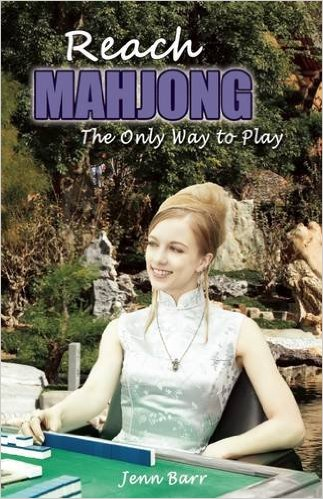
\includegraphics[width=.27\textwidth,clip]{figs/barr1}
\end{center}
\vspace{-50pt}
\end{wrapfigure}

\noindent If you are a complete beginner, I recommend:

\bigskip
\noindent \hspace{10pt}1. Jenn Barr.~2009.~\textit{Reach Mahjong:}\textit{~~~~~~The Only Way to Play.} Huntington Press.
\index{Barr@Barr, Jenn}

\bigskip
\noindent There are a few English books on WWYD (What would you discard) problems. Working on WWYD problems would be a good next step after finishing my book.

\begin{figure}
\begin{center}
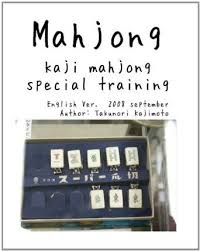
\includegraphics[height=.33\textwidth,clip]{figs/kaji1}
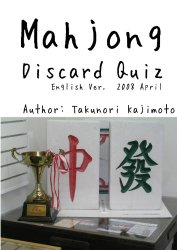
\includegraphics[height=.33\textwidth,clip]{figs/kaji2}
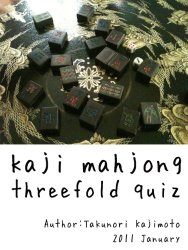
\includegraphics[height=.33\textwidth,clip]{figs/kaji3}
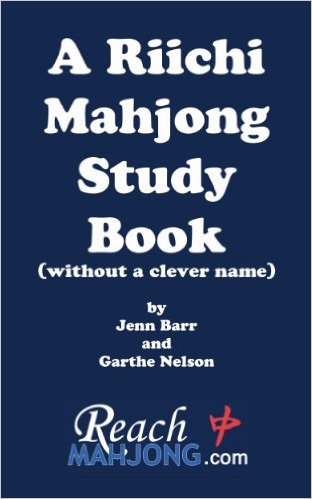
\includegraphics[height=.33\textwidth,clip]{figs/barr2}
\end{center}
\end{figure}



\be \setcounter{enumi}{1}
\i Takunori Kajimoto. 2001. \textit{Mahjong: Kaji Mahjong Special Training.}
\i Takunori Kajimoto. 2008. \textit{Mahjong Discard Quiz.} 
\i Takunori Kajimoto.~2011.~\textit{Mahjong Threefold Quiz.} 
\i Jenn Barr and Garthe Nelson (ed.~Gemma Sakamoto). 2013.~\textit{A Riichi Mahjong Study Book.} Reach Spirits Inc.
\ee \index{Barr@Barr, Jenn}
Of these four books, I recommend the last one, written and edited by three Western professional players with the Japan Professional Mahjong League. The book contains WWYD problems and discussions as well as quizzes about tile efficiency, waits, and score calculation. 

\bigskip
Their WWYD discussions are a lot more multidimensional compared with stylized hand examples introduced in my book. You would find it interesting to see how Jenn and Garthe often disagree about what they would discard. Even those players who share a similar view on strategy principles can still disagree about exactly how to apply these principles in a given situation. 
You would be able to understand their WWYD discussions much better \emph{after} completing my book first. 

\bigskip
Scott D. Miller, a riichi player from Texas, has recently published two books on the history, culture, rules, and variants of riichi mahjong. I have not had a chance to read them, but both of them seem to be a fun reading. 

\vspace{-2pt}
\begin{figure}[h]\centering
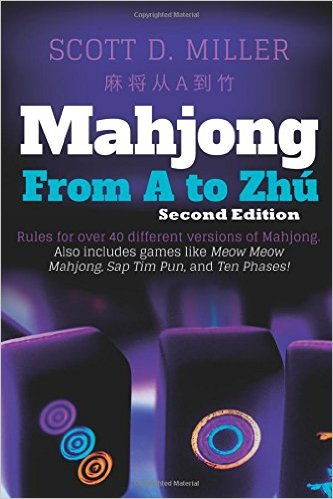
\includegraphics[height=.34\textwidth,clip]{figs/miller1}
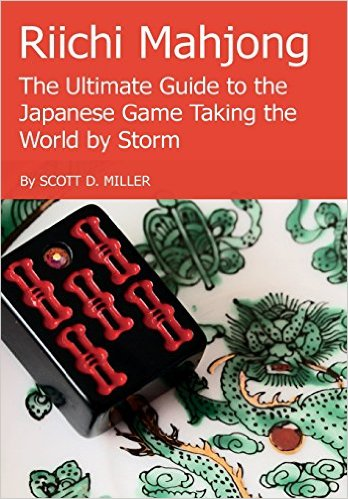
\includegraphics[height=.34\textwidth,clip]{figs/miller2}
\end{figure}
\vspace{-15pt}
\be\itemsep.1em \setcounter{enumi}{5}
\i Scott D. Miller. 2012/2015. \textit{Mahjong From A To Zh\'{u}.} (2nd edition) Lulu.com
\i Scott D. Miller.~2015.~\textit{Riichi Mahjong: The Ultimate Guide to the Japanese Game Taking the World By Storm.} Lulu.com
\ee


\newpage
\section{Online resources}

\subsection*{Osamuko: \url{http://osamuko.com/}} \index{Osamuko}
Osamuko is one of the most extensive online mahjong blogs in English. There are quite a few blog entries there, and many of them are very good. In particular, I find the articles by a contributor named UmaiKeiki very useful. 

\subsection*{Osamuko's Facebook group: \url{https://goo.gl/EMbjwf}}
There is a Facebook group page hosted by one of the contributors of Osamuko. It is a closed group, but I suppose anyone can join the group by sending a request to the administrator. Group members frequently post their play records from {\jap Tenhou} and ask for other members' opinions on them. 

\subsection*{Mahjong on Reddit: \url{https://www.reddit.com/r/Mahjong/}}
Reddit is a social bookmarking website that allows users to add, annotate, edit, and share bookmarks of web documents. It has a lively community dedicated to mahjong where you can discuss mahjong related topics. 

\subsection*{Mahjong News: \url{http://mahjongnews.com/}}
The website is updated regularly with information on upcoming mahjong tournaments (Riichi, MCR, and online), their results, and newly released mahjong books, among other things. 

\subsection*{Japanese Mahjong Wiki: \url{http://arcturus.su/wiki/}}
This website provides an encyclopedic information on rules, terminology, and strategies of riichi mahjong. It is a wiki page so anyone can edit the contents. 

\subsection*{Reach Mahjong of New York: \url{http://mahjong-ny.com/}}
This website not only serves as the hub webpage for players in the US but also provides quite a few useful resources, including a terminology list, beginner's guide, and quizzes about tile efficiency and scoring.

\subsection*{Just Another Japanese Mahjong Blog: \\\url{http://goo.gl/3cKpdI}}
This website has a number of articles on Riichi theories, translated from Chinese. 

\subsection*{ReachMahjong.com: \url{http://reachmahjong.com/en/}}
This website is run by the professional players who wrote the aforementioned Riichi Mahjong Study Book. You can find more WWYD problems and discussions, strategy guides, and reports on tournaments, among other things. 

\subsection*{EMA: \url{http://mahjong-europe.org/}} \index{european@EMA}
This is the official webpage of the European Mahjong Association. You can find information on rules, upcoming tournaments, tournament results and observer reports, and player rankings. 

\subsection*{UKMA: \url{http://ukmahjong.co.uk/}} \index{ukma@UKMA}
This is the official webpage of the UK Mahjong Association. You can find information on the UK Riichi Open tournaments and the affiliated clubs, among other things. 

